% ==============================================================================
% thesis.tex
% Example file for tumthesis.csl
% Michael Ritter, 2012
% Licence:
% This work may be distributed and/or modified under the
% conditions of the LaTeX Project Public License, either version 1.3
% of this license or (at your option) any later version.
% The latest version of this license is in
% http://www.latex-project.org/lppl.txt
% and version 1.3 or later is part of all distributions of LaTeX
% version 2005/12/01 or later.
% ==============================================================================
\documentclass[]{tumthesis}

% ------------------------------------------------------------------------------
%FixMe-Status: final (no FixMe comments) or draft (comments visible)
%\fxsetup{draft}
\fxsetup{final}
% ------------------------------------------------------------------------------

% ------------------------------------------------------------------------------
%  Language selection for metadata and main text (can be changed at any point in
%  the main text.
%\selectlanguage{ngerman}
\selectlanguage{english}
% ------------------------------------------------------------------------------

\def\defSubject{idp}
%working title http://www-m9.ma.tum.de/Allgemeines/WolfgangRiedl
%Darstellung von fortgeschrittenen Graphalgorithmen am Beispiel von Push-Relabel sowie Label-Correcting Algorithmen
\def\defTitle{Visualization of advanced graph algorithms}% using the example of push-relabel as well as label-setting algorithms}

\def\pushRelabel{\texttt{push-relabel}}
\def\maxFlow{\textit{maximum flow problem}}
\def\labelSetting{\texttt{label-setting}}
\def\spprc{\textit{shortest path problem with resource constraints}}

\def\defSubTitle{
\pushRelabel{} algorithm \\ to solve the \maxFlow{} \\
\labelSetting{} algorithm \\ to solve the \spprc{}
}
\def\defProfessor{Prof. Dr. Peter Gritzmann}
\def\defAdvisor{Wolfgang F. Riedl}
\def\defAuthor{Adrian Haarbach}
\def\defDate{December 30, 2016}
\def\defLocation{Munich}
% ------------------------------------------------------------------------------
% Data for the bibliography
\addbibresource{./contents/resources.bib}
% ------------------------------------------------------------------------------

% ------------------------------------------------------------------------------
% Further packages and TikZ libraries can be incorporated here.
\usetikzlibrary{arrows}
% ------------------------------------------------------------------------------

% ------------------------------------------------------------------------------
% Using the include-command: The content of the work will be incorporated using
% the include-command. So that you can test things out without always needing
% the full thesis, you can define here which sections will be incorporated and
% which will not. Of course, for the final version you should be sure to
% incorporate everything.
%\includeonly{%
%%titlepage,%
%%declaration,%
%abstract,%
%introduction,%
%% include own sections here (rule of thumb: one file per chapter)
%conclusion,%
%appendix%
%}%
% ------------------------------------------------------------------------------

% ------------------------------------------------------------------------------
% PDF-Metadaten
\hypersetup{
 pdfauthor={\defAuthor},
 pdftitle={\defTitle},
 pdfsubject={},%\defSubTitle},
 pdfkeywords={},%\subject{\defSubject}},
 colorlinks=true, %coloured links (for the PDF version)
% colorlinks=false, % no coloured links (for the print version)
}
% ------------------------------------------------------------------------------

% ------------------------------------------------------------------------------
% Data for the title page and declaration
\author{\defAuthor}
\title{\defTitle}
\subtitle{\defSubTitle}
\faculty{Fakultät für Mathematik}
\institute{Lehrstuhl für Angewandte Geometrie und Diskrete Mathematik}
%\subject{master}
%\subject{bachelor}
%\subject{diploma}
%\subject{project}
%\subject{seminar}
%\subject{idp}
\subject{\defSubject}
\professor{\defProfessor} %Themensteller
\advisor{\defAdvisor} %Betreuer
\date{\defDate}%\today} %Submission Date
\place{\defLocation} %Place where document is signed
% ------------------------------------------------------------------------------

% ==============================================================================
% Main part of the document
% ==============================================================================
\makeindex[title=Index,options=-s myindex]
\begin{document}
\pagestyle{empty}
\frontmatter%
%\selectlanguage{ngerman}
\selectlanguage{english}
\maketitlepage%
\makedeclaration%

\cleardoublepage
\addcontentsline{toc}{chapter}{Abstract / Zusammenfassung}
\selectlanguage{english}
\section*{Abstract}
This interdisciplinary project deals with the vivid visualization of advanced graph algorithms. In particular, algorithms to solve two distinctive problems in discrete math are considered. Namely the \maxflow{} as well as the \spprc{}. For efficiency reasons, one often employs advanced graph algorithms to solve above problems. The \maxflow{} is solved using the efficient \pushRelabel{}. To solve the \spprc{}, we employ a generic \labelSetting{} which follows the dynamic programming principle.


Both algorithms carry a lot of state variables and are thus not easy to understand intuitively. An additional visualization layer with an intuitive representation of all state variables and state transitions during algorithm execution was developed. It displays the height function of each node in case of the \pushRelabel{} or the pareto frontier of all labels resident in a certain node in case of the \labelSetting{}. To achieve the goal of a high interactivity, we replaced the previous Canvas based graph visualization code with a new implementation based on SVG, using D3.js, a JavaScript library for producing dynamic, interactive data visualizations in web browsers.

%
%This interdisciplinary project deals with the vivid visualization of advanced graph algorithms. In particular, algorithms to solve two distinctive problems in discrete math are considered. For efficiency reasons, one often employs advanced graph algorithms to solve above problems. Both algorithms carry a lot of state variables and are thus not easy to understand intuitively. An additional visualization layer with an intuitive representation of all state variables and state transitions during algorithm execution was developed.
%
%The \maxflow{} is solved using the efficient \pushRelabel{}. It displays the height function of each node. To solve the \spprc{}, we employ a generic \labelSetting{} which follows the dynamic programming principle. The pareto frontier of all labels resident in a certain node is displayed.
% 
%To achieve the goal of a high interactivity, we replaced the previous Canvas based graph visualization code with a new implementation based on SVG, using D3.js, a JavaScript library for producing dynamic, interactive data visualizations in web browsers.


%This IDP aims at extending the previous HTML5 framework that was developed at the chair to support advanced graph algorithms:
%\begin{itemize}
%	\item the Tarjan-Goldberg push-relabel algorithm to solve the maximum flow problem
%	\item a Label Setting algorithm to solve the shortest path problem with resource constraints (SPPRC)
%\end{itemize}
%In particular, the goal was to provide an intuitive visual representation of all state variables and state transitions during the algorithm execution. Since both algorithms carry a lot of state information, an additional visualization layer, linked to the original graph layer was developed. This second layer displays: 
%\begin{itemize}
%	\item the height function of each node in case of the Tarjan-Goldberg algorithm
%	\item the pareto frontier of all labels resident in a certain node in case of the Label Setting algorithm
%\end{itemize}
%
%To achieve the goal of a highly interactive and easily extensible user experience, we replaced the old canvas based graph visualization code, which was really hard to extend, with a new implementation using the Stanford development D3.js (or just D3 for Data-Driven Documents), a JavaScript library for producing dynamic, interactive data visualizations in web browsers. It makes use of the widely implemented SVG, HTML5, and CSS standards. 
%
%During the development process, we also migrated the existing graph editor to the new technologies, it now easily supportsan arbitrary number of resources defined on edges and nodes download and upload functionality cropped SVG export of graphs
%
%This talk is not only suitable to mathematicians found of graph problems, but to anyone who wants to leverage today's web standards to express his interactive visualization needs.
%

\selectlanguage{ngerman}
\section*{Zusammenfassung}
Das vorliegende interdisziplinäre Projekt beschäftigt sich mit der anschaulichen Darstellung von fortgeschrittenen Graphalgorithmen. Betrachtet werden zwei Verfahren zur Lösung von Problemstellungen der diskreten Mathematik. Die zu visualisierenden Problemstellungen sind hierbei das \maxflowDE{} sowie das \spprcDE{}. Als Lösungsverfahren für die aufgeführten Problemstellungen werden aus Effizienzgründen häufig fortgeschrittene Graphalgorithmen herangezogen. Für die Lösung des \maxflowDEGen{} findet der bekannte \pushRelabelDE{} in der Praxis häufig Anwendung. Zur Lösung des \spprcDEGen{} wird mit einem \labelSettingDE{} ein bekanntes Verfahren der dynamischen Programmierung vorgestellt.


Beide Algorithmen führen eine Menge an Statusvariablen mit sich und sind deshalb nicht leicht intuitiv zu verstehen. Es wurde eine zusätzliche Visualisierungsebene mit intuitiver Repräsentation aller Statusvariablen und -übergänge entwickelt. Diese veranschaulicht die Höhenfunktion jedes Knotens im Falle des \pushRelabelDE{} oder dessen Pareto-Front im Falle des \labelSettingDE{}. Um hohe Interaktivität zu erreichen, ersetzten wir den bisherigen auf Canvas basierenden Graphen-Visualisierungscode mit einer neuen Implementierung basierend auf SVG mit D3.js, eine JavaScript Bibliothek zur Erzeugung dynamischer, interaktiver Datenvisualisierungen in Web Browsern.
%Das interdisziplinäre Projekt hat das Ziel, die erwähnten Problemstellungen mit einfachen Worten zu erklären und durch Beispiele zu motivieren sowie die verwendeten Lösungsverfahren graphisch zu veranschaulichen. Die Darstellung wird hierbei in Form einer separaten Web-Applikation für jede Problemstellung erfolgen, welche aus Gründen der einheitlichen Darstellung und der der leichteren Wartbarkeit auf ein gemeinsames, bereits existierendes Framework aufbauen wird.

\selectlanguage{english}
\tableofcontents%

\mainmatter%
\pagestyle{headings}

\chapter{Introduction}\label{ch:1}

Most previous visualizations of graph algorithms \cite{storz2013idp,velden2014idp,sefidgar2015idp,becker2015idp,zoennchen2015idp,fischer2016idp,feil2016idp} are based on displaying the state of the algorithm on top of a network visualization of a graph, e.g. by annotating vertices or edges with additional information.

For advanced graph algorithms \cite{goldberg1988new,irnich2005shortest}, which are often employed for efficiency reasons, the state size to visualize may become quite large. It may be thus advantageous to visualize the state of such algorithms in an additional visualization layer. 

The ideas of these visualizations have long existed in a static form in textbooks describing the theory behind these algorithms with specific examples. Nevertheless, we are unaware of a dynamic visualization of these additional state variables.

\section{Related work}
\section{Contributions}
In addition to the two applications of advanced graph algorithms related to m

\section{Overview}

\chapter{Background}\label{ch:2}
Problems defined on networks arise in many real-life applications. A network can mathematically be represented by a graph. 

\newcommand{\Ein}[1]{\delta^-(#1)}
\newcommand{\Eout}[1]{\delta^+(#1)}
\newcommand{\ein}{{e_{\text{in}}}}
\newcommand{\eout}{{e_{\text{out}}}}

%for algorithms
%\newcommand{\setfont}[1]{\mathcal{#1}}
\newcommand{\setfont}[1]{#1}

%\section{math}
\begin{definition}[simple directed graph]
A graph is an ordered pair $G = (V, E)$ consisting of a vertex (or node) set $V$ and an edge (or arc) set $E$. The unqualified term "graph" usually refers to a \textit{simple} graph which has no multiple edges or self-loop edges. In a \textit{directed graph (digraph)}, $E$ is a set of ordered pairs of vertices, a subset of the cartesian product of vertices, that is $E \subseteq V \times V$. If the graph is simple, each edge $e \in E$ can be uniquely identified by a pair of vertices from $V$, that is $e=(v,w)$ with $v,w \in V$ and $v \neq w$, where $v$ is the start vertex and $w$ is the end vertex of the directed edge or arc $e$ \cite{jungnickel2013graphs}[1.6]. \end{definition}

\begin{figure}
\centering
	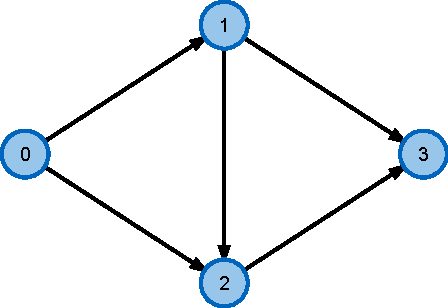
\includegraphics{fig/graph-editor}
	\caption{a digraph with $V=\{0,1,2,3\}$, $E=\{(0,1),(0,2),(1,2),(1,3),(2,3)\}$}
	\label{fig:graph}
\end{figure}

For problems and algorithms defined on digraphs, it is often convenient to define the set of edges coming into a vertex $v$ and the set of edges leaving it:
\begin{align}
\Ein{v}  &: \{ e=(u,v) \in E \; | \; u,v \in V \} \eqname*[eq:incoming]{incoming edges} \\
\Eout{v} &: \{ e=(v,w) \in E \; | \; v,w \in V \} \eqname*[eq:outgoing]{outgoing edges} \\
\nonumber
\end{align}
In above example of a digraph \refFigure{fig:graph}, the vertex $v=2$ has an incoming edge set of $\Ein{2}=\{(0,2),(1,2)\}$ and an outgoing edge set of $\Eout{2}=\{(2,3)\}$.

\newpage
%\section{computer science}
Advanced algorithms to solve graph problems rely on common programming principles. The first one is so basic that it actually forms the basis of sorting algorithms such as \textit{MergeSort}.
\begin{definition}[divide-and-conquer]
\textit{In divide-and-conquer, we solve a problem recursively, applying three steps at each level of the recursion:
\textbf{Divide} the problem into a number of subproblems that are smaller instances of the same problem. 
\textbf{Conquer} the subproblems by solving them recursively. If the subproblem sizes are small enough, however, just solve the subproblems in a straightforward manner. 
\textbf{Combine} the solutions to the subproblems into the solution for the original problem.} \cite[ch. 4]{cormen2009introduction}
\end{definition}

Recursion is clear and appealing from a mathematical perspective, but for computational efficiency reasons, divide-and-conquer is not always the best choice. It is better to remember useful intermediate results.
%\begin{definition}[recurrence]
%A recurrence relation is a mathematical formulation of the divide-and-conquer paradigm, an equation or inequality that descibes a function recursively in terms of base case and 
%\end{definition}

\begin{definition}[dynamic programming]
\textit{Dynamic programming, like the divide-and-conquer method, solves problems by combining the solutions to subproblems. %(“Programming” in this context refers to a tabular method, not to writing computer code.) 
[...] divide-and-conquer algorithms partition the problem into disjoint subproblems, solve the subproblems recursively, and then combine their solutions to solve the original problem. In contrast, dynamic programming applies when the subproblems overlap - that is, when subproblems share subsubproblems. In this context, a divide-and-conquer algorithm does more work than necessary, repeatedly solving the common subsubproblems. A dynamic-programming algorithm solves each subsubproblem just once and then saves its answer in a table, thereby avoiding the work of recomputing the answer every time it solves each subsubproblem.} \cite[ch. 15]{cormen2009introduction} 
%\cite[ch. 3, p. 70]{ahuja1993network}
\end{definition}
Dynamic programming can be applied to a wide range of graph problems, as we will see later. It works because of Bellman's:
\begin{definition}[Principle of Optimality]
\textit{An optimal policy has the property that whatever the initial state and initial decision are, the remaining decisions must constitute an optimal policy with regard to the state resulting from the first decision} \cite[sec. 3.3]{bellman1957dynamic}.
\end{definition}

For some kind of problems, we can get even more efficient with the greedy approach originating from matroid theory \cite[sec. 13.7, p. 528]{ahuja1993network} \cite[ch. 5]{jungnickel2013graphs}. It is at the heart of the efficient and well known Dijkstra algorithm.
\begin{definition}[greedy]
\textit{Algorithms for optimization problems typically go through a sequence of steps, with a set of choices at each step. For many optimization problems, using dynamic programming to determine the best choices is overkill; simpler, more efficient algorithms will do. A greedy algorithm always makes the choice that looks best at the moment. That is, it makes a locally optimal choice in the hope that this choice will lead to a globally optimal solution.} \cite[ch. 16]{cormen2009introduction}
\end{definition}

\chapter{Background}\label{ch:3}
This chapter mathematically formalizes the problems we consider in this work as well as the algorithms used to solve these problems. We start with the basic definition of a graph and then look at different problems that can be defined on them. Finally, we  

Problems defined on networks arise in many real-life applications. A network can be represented by a graph.

\newcommand{\Ein}[1]{\delta^-(#1)}
\newcommand{\Eout}[1]{\delta^+(#1)}
\newcommand{\ein}{{e_{\text{in}}}}
\newcommand{\eout}{{e_{\text{out}}}}

\begin{definition}[directed graph]
A graph is an ordered pair $G = (V, E)$ consisting of a vertex (or node) set $V$ and an edge (or arc) set $E$. In a \textit{directed graph (digraph)}, $E$ is a set of ordered pairs of vertices, a subset of the cartesian product of vertices, that is $E \subseteq V \times V$. Thus, each edge $e \in E$ can be uniquely identified by a pair of vertices from $V$, that is $e=(v,w)$ with $v,w \in V$ and $v \neq w$, where $v$ is the start vertex and $w$ is the end vertex of the directed edge or arc $e$ \cite{jungnickel2013graphs}[1.6]. For problems or algorithms defined on digraphs, it is often convenient to define the sets of edges coming into a vertex $v$ or leaving it.
\begin{align}
\text{incoming edges} \quad \quad \Ein{v}  &: \{ e=(u,v) \in E \; | \; u,v \in V \}  \\
\text{outgoing edges} \quad \quad \Eout{v} &: \{ e=(v,w) \in E \; | \; v,w \in V \}
\end{align}
\end{definition}


\section{The \maxflow{}}
An important problem in many applications is to find out the maximum amount of flow that can simultaneously be transferred over a network between two points. % from $s$ to $t$. 
Depending on the context, flow can mean different things, e.g the amount of water in a water pipe system in your city or the bandwidth of a computer network. We call such a network a \textit{flow network}:

\begin{definition}[flow network]
A \textit{flow network} $N$ is a 4-tuple $N=(G,c,s,t)$ consisting of \textit{digraph} $G$, a positive real-valued capacity function $c: E \rightarrow \mathbb{R}_+ , \forall e \in E : c(e) \geq 0$ defined on all edges of the graph and two designated vertices, the \textit{source} $s \in V$ and \textit{sink} (or target) $t \in V$ \cite{ahuja1993network}[1.2].
\end{definition}


%However, the links in the network on paths from $s$ to $t$ can only handle flow up to their maximum capacity $c$. One now seeks an assignment of flow values $f$ to edges $e$ that fulfills all the capacity constraints of the edges and the flow conservation property on all the inner nodes, meaning we don't want leaks in our pipe system.
However, the individual links in the network can only handle flow up to their maximum capacity, e.g. they are limited by the thickness of the water pipe. Additionally, the total flow must be preserved at the intermediate joints, e.g. we don't want leaks in our pipe system. This is called a \textit{feasible flow}:% Given such a network, an obvious problem is to find out the maximum amount of flow that can simultaneously be transfered over the network, 


\begin{definition}[feasible flow]
A \textit{feasible flow} $f$ from $s$ to $t$ is a mapping $f : E \rightarrow \mathbb{R}$ satisfying two constraints: The \Eqref{eq:cap} ensures that the flow over an edge is always positive and not exceeding the edge's maximum capacity, while the \Eqref{eq:conserv} assures that the total flow into a vertex $v \notin {s,t}$ equals the total flow out of $v$:
\begin{align}
\forall e \in E &: 0 \leq f(e) \leq c(e) \eqname*[eq:cap]{capacity constraint} \\
\forall v \in V \setminus \{s,t\} &: \sum_{e \in \Ein{v}} f(e) = \sum_{e \in \Eout{v}} f(e) \eqname*[eq:conserv]{flow conservation} \\ \nonumber
\end{align}
\end{definition}

There might be many feasible flows (e.g the zero flow $f = 0 \, \forall e \in E$), but we are especially interested in transferring as much as possible across the network, the \textit{maximum flow}:
\begin{problem}[maximum flow]
A \textit{maximum flow} $\max \abs{f}$ is a \textit{feasible flow} that maximizes the \textit{flow value} $\abs{f}$, the amount of flow which flows from $s$ to $t$. This is the net flow into the sink $t$ or out of the source $s$:
\begin{equation*}
\abs{f} = \sum_{e \in \Ein{t}} f(e) = \sum_{e \in \Eout{s}} f(e)
\end{equation*}
\end{problem}


An important concept in the context of flow algorithms is the residual network capturing possible change to $f$, defined by the residual capacities $c'$ and the \textit{residual graph} $G'$:
\begin{definition}[residual graph]
For a flow $f$ in $G=(V,E)$, we can construct the \textit{residual graph} $G' = (V,E')$ by copying all the vertices $v \in V$ from $G$ and for each $e \in E$ adding one or two edges $e'$ to $E'$ with \textit{residual capacity} $c'$ under the following rules \refFigure{fig:residual}:
\begin{description}
\item[forward edge] if $f(e) < c(e)$ for an edge $e=(a,b) \in E$, then add the forward edge $e' = (a,b)$ with residual capacity $c'(e') = c(e) - f(e)$ to $E'$.
\item[backward edge] if $f(e) > 0$ for an edge $e=(a,b) \in E$, then add the backward edge $e' = (b,a)$ with residual capacity $c'(e') = f(e)$ to $E'$.
\end{description}
\end{definition}

\begin{figure}
\centering
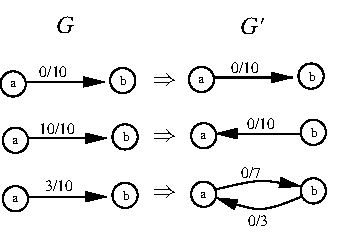
\includegraphics[]{fig/residual}
\caption{Construction of the residual graph $G'$ \cite{mayer2013prakt}.}
\label{fig:residual}
\end{figure}



\section{The \spprc{}}
Another basic problem defined on networks is how to traverse a network to get from one point to another one as cheaply as possible. For this problem we wish to find a shortest path between two points.

\begin{definition}[path]
A \textit{path} $P = (e_1, e_2, ... e_p)$ is a finite sequence of arcs (some arcs may occur more than once) where the end vertex of $e_i \in E$ is identical to the start vertex of $e_{i+1} \in E$ for all $i=1,\dots,p-1$. For simple graphs, a path can be also be written as $P = (v_0,v_1,\dots,v_p)$ since the edges can be uniquely idetified by start and end vertex $e_i=(v_{i-1},v_i)$. The length of a path is $p$ \cite{irnich2005shortest}.
\end{definition}


The ordinary shortest path problem (SPP) is perhaps the simplest of all network problems. It seeks an (unconstrained) $s$-$t$ path of minimal cost (or length) between two points. A real-valued cost function $c : E \rightarrow \mathbb{R}$ is defined on all edges of the graph. The cost or length of a path is defined as the sum of the costs of all the edges along the path, that is $c(P)=\sum_{i=1}^p c(e_i)$. \\



In the shortest path problem with resource constraints (SPPRC), each edge additionally carries a secondary (possibly higher-dimensional) resource vector or function $r$. A path $P$ is now constrained at the intermediate vertices $v_i$ with lower and upper bounds on the accumulated resource consumptions along the (partial) paths.\\

\begin{example}[SPPTW]
An illustrative example is the two-resource SPPRC, the shortest path problem with time windows (SPPTW). In addition to the \textit{cost} $c$, each edge additionally bears the resource \textit{time} $t$. Thus each edge is associated with the two-dimensional resource vector $(t,c) \forall e \in E$. The secondary resource \textit{time} is constrained, while the primary resource \textit{cost} is unconstrained, but seeks to be minimized.

The accumulated consumptions of the resource \textit{time} along a path are constrained at the intermediate vertices along that path by lower and upper limits, that is the earliest arrival time $t_a$ and the latest departure time $t_b$ and called the \textit{resource window}, denoted as a tuple $[t_a,t_b] \forall v \in V$.
\end{example}

$[t_{arrival},t_{departure}] \forall v \in V$



\chapter{Shortest paths}\label{ch:4}

\section{The \spprc{}}
Another basic problem defined on networks is how to traverse a network to get from one point to another one as cheaply as possible. For this problem we wish to find a shortest path between two points.

\begin{definition}[path]
A \textit{path} $P = (e_1, e_2, ... e_p)$ is a finite sequence of arcs (some arcs may occur more than once) where the end vertex of $e_i \in E$ is identical to the start vertex of $e_{i+1} \in E$ for all $i=1,\dots,p-1$. For simple graphs, a path can be also be written as $P = (v_0,v_1,\dots,v_p)$ since the edges $e_i=(v_{i-1},v_i)$ can be uniquely identified by the start and end vertex. The length of a path is $p$ \cite{irnich2005shortest}.
\end{definition}


\begin{definition}[SPP]
The ordinary shortest path problem (SPP) is perhaps the simplest of all network problems. It seeks an (unconstrained) $s$-$t$ path of minimal cost (or length) between two points. A real-valued cost function $c : E \rightarrow \mathbb{R}$ is defined on all edges of the graph. The cost of a path is defined as the sum of the costs of all the edges along the path, that is $c(P)=\sum_{i=1}^p c(e_i)$. The problem exists in two variants: shortest paths from a single source (APSP) or between all pairs (APSP) of vertices.
\end{definition}

\begin{definition}[SPPRC]
A possible generalization of the SPP is the shortest path problem with resource constraints (SPPRC), where each edge additionally carries a secondary (possibly higher-dimensional) resource vector or function. A path $P$ is now constrained at the intermediate vertices $v_i$ with lower and upper bounds on the accumulated resource consumptions along the (partial) paths.
\end{definition}

\begin{definition}[SPPTW]
An illustrative example is the two-resource SPPRC, the shortest path problem with time windows (SPPTW). In addition to \textit{cost} $c$, each edge additionally bears the resource \textit{time} $t$. Thus each edge is associated with the two-dimensional resource vector $(t,c) \, \forall e \in E$. The secondary resource \textit{time} is constrained, while the primary resource \textit{cost} is unconstrained, but seeks to be minimized. The accumulated consumptions of the resource \textit{time} along a path are constrained at the intermediate vertices along that path by lower and upper limits, that is the earliest arrival time $t_a$ and the latest departure time $t_b$ and called the \textit{resource window}, denoted as tuples $[t_a,t_b] \, \forall v \in V$. The objective of the SPPTW is to find paths $P=(v_0=s,v_1,v_2,\dots,v_n=t)$ such that 
\begin{itemize}
	\item $\forall v_j \in P: arr(v_j) \leq \sum_{i=1}^{j}{time(v_{i-1},v_{i})} \leq dep(v_j)$
	\item $cost(P) = \min{\sum_{i=1}^{n}cost(v_{i-1},v_i)}$
\end{itemize}
\end{definition}



\section{\labelSetting{}}
We start with the distinction between label-setting \cite[ch. 4]{ahuja1993network} and label-correcting \cite[ch. 5]{ahuja1993network} algorithms that solve the ordinary shortest path problem (SPP).
The first label-setting algorithm was suggested by Dijkstra \cite{dijkstra1959note}\footnote{secondary sources \cite[sec. 4.5]{ahuja1993network},\cite[sec. 24.3]{cormen2009introduction},\cite[sec. 3.7, p. 83]{jungnickel2013graphs}}. It solves the SSSP with non-negative edge weights and is visualized in \cite{velden2014idp}. Its runtime is $O(|V|^2)$ which can further be improved to $O(|E| + |V| \log |V|)$ when using a Fibonacci heap for the queue of active nodes. After a node has been processed, the distance label of the path ending in that node is permanent and will thus not change in subsequent iterations. The algorithm is a greedy method and is thus very efficient.
On the other hand, label-correcting algorithms allow negative edge weights and can detect negative cycles. Labels stay temporary until the very end of the algorithm execution. An example which solves the SSSP with negative edge weights is the Bellman-Ford algorithm \cite{bellman1958routing,ford1962flows}\footnote{secondary sources \cite[sec. 5.4]{ahuja1993network},\cite[sec. 24.1]{cormen2009introduction},\cite[sec. 3.7, p. 87]{jungnickel2013graphs}}. It has a runtime of $O(|V|\cdot|E|)$ and is visualized in \cite{storz2013idp}. An example which solves the APSP is the Floyd-Warshall algorithm \cite{floyd1962algorithm,warshall1962theorem}\footnote{secondary sources \cite[sec. 5.6]{ahuja1993network},\cite[sec. 25.2]{cormen2009introduction},\cite[sec. 3.9]{jungnickel2013graphs}} with a runtime of $O(|V|^3)$ and it is visualized in \cite{becker2015idp}. These two algorithms are dynamic programming approaches. 

%, which are either label setting or label correcting algorithms. 
The recent survey \cite{irnich2005shortest} gives an overview of algorithms for the solution of shortest path problems with resource constraints (SPPRC). They provide a generic SPPRC algorithm based on dynamic programming. Depending on the path selection strategy, the generic algorithm results in a label setting or label correcting algorithm. We choose the simplest variant of the SPPRC, the shortest path problem with time windows (SPPTW), sometimes also called the vehicle routing problem with time windows (VRPTW). The underlying network must either be acyclic or the resource consumptions for at least one resource must be strictly positive along a path to allow for a label-setting algorithm. 

An optimal solution of the full problem consists of optimal solutions of partial problems, that is, the shortest s-t path with time window constrains contains optimal shortest partial paths s-v for all v on the shortest s-t path. This optimality principle of Bellman \cite{bellman1957dynamic} can be written as a dynamic programming recursion for time-windows $[t_a,t_b] \, \forall v \in V$ and resource vectors $(t,c) \, \forall e \in E$:
\begin{align*}
	T(P_0) &= t_a^0 \\
	T(P_i) &= \max\{t_a^i, T(P_{i-1}) + t_i\}
\end{align*}
Here, $T$ stands for the accumulated consumption of the resource time $t$ along the edges of a path $P$. In the recursion case, we take the maximum of earliest arrival time $t_a$ and accumulated time consumption of the prefix path $P_{i-1}$ extended along the current edge $e$, $T(P_{i-1}) + t_i$, because waiting at a node is allowed.

Fortunately, not all of the dynamic programming partial results are kept. First of all, it can be the case that $T(P_{i-1}) + t_i > t_b^i$. This means that the time window at the node is exceeded. The path or label obtained from above extension is \textit{infeasible} and thus discarded.

Secondly, path or labels who are feasible, but equal or worse in both time and cost than other feasible labels can be discarded. A label \textit{dominates} all labels in its right upper cone in the chart of cost/time. The set of all such labels is \textit{pareto-optimal}. Even though we will finally be interested in feasible, minimum cost labels ending in t, we cannot discard any of them at intermediate nodes since extensions of one label with lower cost but higher time might have unfeasible extensions at subsequent vertices along the paths while others with higher cost and lower time don't. 


%\documentclass[a4paper,11pt]{article}
%\usepackage[linesnumbered,ruled,vlined]{algorithm2e}
%%\newcommand{\setfont}[1]{\mathcal{#1}}
%\newcommand{\setfont}[1]{#1}
%\begin{document}

\begin{algorithm}[h!]
\DontPrintSemicolon % Some LaTeX compilers require you to use \dontprintsemicolon instead
\KwIn{directed Graph $G=(V,E)$ with
\begin{itemize}
	\setlength\itemsep{0pt}
	\setlength{\parskip}{0pt}
	\item $\forall$ nodes $v \in V$: [arrive, depart] time window resource constraint
	\item $\forall$ edges $e \in E$: (time,cost) 2-dimensional resource consumptions
	\item start Node $s$, end Node $t$
\end{itemize}}
\KwOut{feasible, pareto-optimal $s \rightarrow t$ paths} \vspace{0.2cm}
(* Initialize *) \;
SET $\setfont{U} = \{(s)\}$ and $\setfont{P} = \emptyset$ \;
\While{$\setfont{U} \neq \emptyset$}{
	(* Path extension step *)\;
	CHOOSE a path $\setfont{Q} \in \setfont{U}$ and REMOVE $\setfont{Q}$ from $\setfont{U}$\;
	\ForAll{arcs $(v(\setfont{Q}), w) \in A$ of the forward star of $v(\setfont{Q})$}{
		\If{$(\setfont{Q},w) \in \setfont{F}(s,w) \cap \setfont{G}$}{
			ADD $(\setfont{Q},w)$ to $\setfont{U}$
		}
	}
	ADD $\setfont{Q}$ to $\setfont{P}$\;
	(* Dominance step *)\;
	\If{(* any condition *)}{
		APPLY dominance algorithm to paths from $\setfont{U} \cup \setfont{P}$ ending at some node $v$\;
	}
}
(* Filtering step *)\;
FILTER $\setfont{P}$, i.e., identify a solution $\setfont{S} \subseteq \setfont{P}$\;
\caption{Generic Dynamic Programming SPPRC Algorithm}
\end{algorithm}


%\end{document}
In our visualization concept \refFigure{fig:spprc}, we show how paths are extended and discarded. The primary visualization layer displays the graph network, the 2-dimensional resource vector of an edge and the time-window at the vertices. Paths can be highlighted. The secondary visualization layer displays the corresponding labels in a 2-dimensional chart, where the axis are cost/time. It also displays the time window of the current node as a rectangle. The labels to be displayed can be filtered by their resident nodes by clicking on it, which allows to view the pareto-frontier of a node. By clicking on a label, the corresponding path is highlighted. Meaningful default filters are implemented depending on the state of the algorithm execution.
\begin{figure}
\centering
\begin{subfigure}[t]{0.45\textwidth}
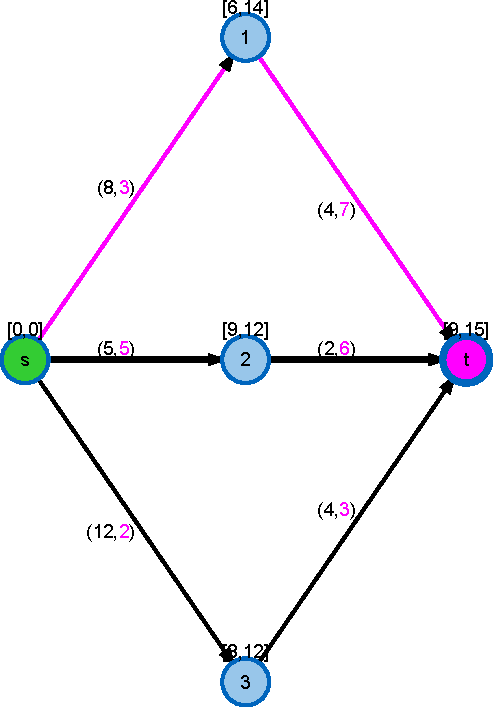
\includegraphics[width=\textwidth]{fig/spp-rc-graph-algorithm-graph}
\end{subfigure}
\begin{subfigure}[t]{0.45\textwidth}
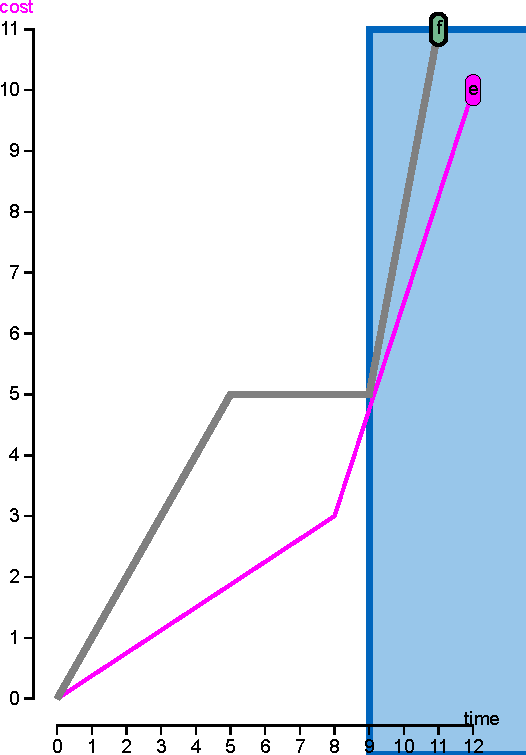
\includegraphics[width=\textwidth]{fig/spp-rc-graph-algorithm-labels}
\end{subfigure}
\caption{spprc concept}
\label{fig:spprc}
\end{figure}



\chapter{Implementation}\label{ch:5}

\newenvironment{ssfont}{\fontfamily{lmss}\selectfont}{\par}

The implementation is an evolution of previous web applications for the visualization of graph algorithms \cite{storz2013idp,velden2014idp,sefidgar2015idp,becker2015idp,zoennchen2015idp}. However, the requirements for graphs with arbitrary resources, a secondary visualization layer and high interactivity urged us to reimplement large parts of the existing codebase using different technologies \refSec{sec:technologies} while still maintaining the same look and feel. In the process, a complete understanding of the interplay between the different components was acquired, which allowed us to refactor them systematically to achieve a better software design \refSec{sec:design}. %This chapter concludes with an installation or deployment manual for the developed web applications \refSec{sec:installation}.

\section{Web technologies}\label{sec:technologies}
Web technologies form the basis of our implementation. The Mozilla Developer Network (MDN)\footnote{\url{https://developer.mozilla.org/docs/Web}} is an excellent reference, which subdivides the technologies into basics \refSec{sec:basic}, scripting \refSec{sec:script} and graphics \refSec{sec:graphics}. Furthermore, we use two JavaScript Software libraries \refSec{sec:libraries} to facilitate certain tasks.

\subsection{Basics: HTML, CSS, HTTP and AJAX}\label{sec:basic}
The HyperText Markup Language (HTML) is used to define the static \textit{content} of the webpage. Each webpage contains just one HTML file, \texttt{\href{http://www.adrian-haarbach.de/idp-graph-algorithms/implementation/maxflow-push-relabel/index_en.html}{maxflow-push-relabel/index\_en.html}} or \texttt{\href{http://www.adrian-haarbach.de/idp-graph-algorithms/implementation/spp-rc-label-setting/index_en.html}{spp-rc-label-setting/index\_en.html}}, for all its static content. These serve as the entry point for our single-page web application and contain all language-specific features. For localization purposes one needs to modify only this file. Cascading Style Sheets (CSS) are used to describe the \textit{appearance or presentation} of the content on the webpage. They can be used both for HTML (\texttt{\href{http://www.adrian-haarbach.de/idp-graph-algorithms/implementation/library-d3-svg/css/style.css}{library-d3-svg/css/style.css}}) and for SVG Graphics such as our graph (\texttt{\href{http://www.adrian-haarbach.de/idp-graph-algorithms/implementation/library-d3-svg/css/graph-style.css}{library-d3-svg/css/graph-style.css}}). The Hypertext Transfer Protocol (HTTP) is used to deliver HTML and other hypermedia documents on the Web. The basic files we need everywhere are statically linked from within our HTML page with \texttt{<link href="...">} for CSS and \texttt{<script src="...">} for JavaScript files. By using asynchronous JavaScript and XML (AJAX) we can issue HTTP requests dynamically, for example when selecting another sample graph, without the need to completely reload the entire page.

\subsection{Scripting: JavaScript, DOM, Web APIs, HTML5 and Node.js}\label{sec:script}
JavaScript is the scripting language that runs natively in a browser. It was originally developed to  add interactivity and other dynamic features to a webpage. This is achieved by manipulating the Document Object Model (DOM), a programming interface for HTML, XML and SVG documents. It provides a structured representation of the document as a tree which can be modified and extended using JavaScript and other languages. The JavaScript language contains standard built-in global objects, e.g. the JSON\footnote{\url{https://developer.mozilla.org/docs/Web/JavaScript/Reference/Global_Objects/JSON}} object with methods for parsing JavaScript Object Notation (JSON), used for serialization of algorithm state to provide the replay functionality. Web Application Programming Interfaces (Web APIs) complement the standard built-in global objects to provide a way to access the browser's advanced functionality programmatically. We make use of this functionality to serialize and download dynamically generated SVG using \texttt{XMLSerializer.serializeToString()}\footnote{\url{https://developer.mozilla.org/docs/Web/API/XMLSerializer}} and \texttt{WindowBase64.btoa()}\footnote{\url{https://developer.mozilla.org/docs/Web/API/WindowBase64}} and we make use of the \texttt{FileReader.readAsText()}\footnote{\url{https://developer.mozilla.org/docs/Web/API/FileReader}} for the local graph upload functionality. Because of their importance, the APIs and the DOM are now fundamental parts of the new HTML5 specification, which extends the HTML markup with new syntactic features such as \texttt{<video>, <audio>, <canvas>} and \texttt{<svg>} tags and the support for mathematical formulas with MathML markup.

\subsubsection{Server-side scripting using Node.js} % only the specific parts we just discussed above. The standard for JavaScript is defined as ECMAScript. As such, 
However, the JavaScript language itself is not restricted to client-side scripting in the browser, it can also be used for server-side scripting using the Node.js host environment. Nowadays there is a huge JavaScript ecosytem consisting of different open-source packages that allow to use JavaScript for all kinds of programming. We used NPM as package manager and Grunt as build tool to implement a simple web-server for development purposes. This circumvents some browsers' security settings of disallowing AJAX requests when files are served locally, which would prohibit us from loading different graphs.\footnote{In fact, this restriction is only present in Google Chrome and can be circumvented when starting it with the \texttt{-{}-allow-file-access-from-files} flag. The latest versions of Firefox and Safari don't seem to have this restriction anymore as it was already observed by \cite{feil2016idp}. Another alternative would be to install a production-quality web-server such as Apache, but this is overkill during development.}

\subsubsection{JavaScript - a fully featured programming language}
JavaScript is not just a lightweight scripting language, it is actually a fully featured programming language. It has matured a lot during its standardization process (ECMAScript), a complete reference is given by \cite{flanagan2011javascript}. It is an interpreted, prototype-based, multi-paradigm dynamic scripting language with first-class functions. It supports imperative, object-oriented, and declarative or functional programming styles. As such, it is actually superior to more traditional languages such as Java or C++, which only made a functional programming style possible in their latest editions of Java 7 and C++ 11 through \textit{lambdas}. The object-oriented part of JavaScript works a little different than in the traditional languages, because it relies on prototype object based inheritance instead of class based inheritance. A good introduction to the language suitable for beginners covering the important concepts of scope and closure of the functional style and prototypal-based inheritance of the object-oriented style is given by \cite{haverbeke2015eloquent,resig2013secrets}.
While being an incredibly expressive and flexible language, the original creators of JavaScript initially made a few bad design decisions, but it is too late to remove them completely from the language nowadays. This is why it has become the \textit{world's most misunderstood programming language} according to Douglas Crockford, whose advice is to stick to \textit{JavaScript: The Good Parts} \cite{crockford2008javascript}, which is the title of his advanced book about the language features one should use and the ones to be avoided.
Since we partly follow the object-oriented programming style to create reusable software components, we had to deal with good software design, which will be covered later \refSec{sec:design}. To harness the full power of JavaScript effectively, e.g. with statics, singletons and different code-reuse patterns, we recommend \cite{herman2012effective}.

\subsection{Graphics: SVG vs. Canvas}\label{sec:graphics}
SVG and Canvas are part of HTML5 and both are used to display interactive graphics on a webpage. 
The previous interdisciplinary projects were based on \textbf{Canvas}, which allows for dynamic, scriptable rendering of \textit{raster-based} 2D graphics using JavaScript. It is a \textit{low-level}, procedural model that updates a bitmap pixel by pixel using drawing routines. Once an object is drawn, it is forgotten by the browser. The complete scene thus has to be redrawn after any changes. The quality of the resulting bitmap is resolution dependent, leading to poor text rendering and scaling capabilities. 
On the other hand, Scalable Vector Graphics (\textbf{SVG}) is a \textit{high-level} language for describing \textit{vector-based} 2D graphics using XML notation, in complete analogy to HTML which describes page layout using XML notation. Similar to the HTML DOM which allows to access individual nodes of the page tree, individual shapes of the vector graphic can be accessed and modified via an SVG DOM, the scene graph. This allows to modify and re-render only a subset of the scene. Furthermore, it allows to attach JavaScript event handlers to individual shapes, easing interaction capabilities like clicks on nodes and edges or resources in our graph editor. Because of its advantages over Canvas, the previous interdisciplinary projects have lately been migrated to SVG \cite{feil2016idp} and all current projects \cite{feil2016idp,fischer2016idp} already use our beta SVG implementation, profiting from its new features.

\subsubsection{Arrowhead markers for directed edges}
SVG primitives such as \texttt{circle} and \texttt{line} are used to represent a graph. For digraphs, we need directed arrows. These can be added to a line by setting its \texttt{marker-end} style to a  previously defined marker url, e.g. \texttt{url(\#arrowhead2)}. The marker definition is:\\
{\footnotesize{\texttt{<marker id="arrowhead2" refX="24" refY="4" markerUnits="userSpaceOnUse" markerWidth="24" \\ markerHeight="8" orient="auto"><path d="M 0,0 V 8 L12,4 Z"></path></marker>}}}

At its core is the path element defining a filled triangle using SVG's mini plotting language: \texttt{M 0,0} (move to the origin), \texttt{V 8} (draw a vertical line up to 8,0), \texttt{L12,4} (then a line to 12,4, which is the tip of the arrow/triangle), \texttt{Z} (go back to the origin and fill the resulting polygon). By using {\footnotesize\texttt{orient="auto-start-reverse"}} we can get arrows in the reverse direction, which we use to display backward edges of the residual graph using just the original edge.
The concurrent project \cite{feil2016idp} used an early version of our implementation which had the limitation that the marker definition was defined in the HTML page for each combination of arrow size and colour. We now removed most of the shortcomings. By using {\footnotesize\texttt{markerUnits="userSpaceOnUse"}} the size of the marker is independent of the line thickness, which previously led to misplaced and oversized markers when a line was highlighted by drawing it thicker. Above code is added dynamically via JavaScript to an invisible SVG element on the webpage so that we don't need to define it in HTML, easing reuse.\footnote{It is important that the same definition exists only once per web page and not once per SVG element, because otherwise Firefox does not render the arrows correctly. Chrome however is unaffected by this.}

%Nachteil der gewa ̈hlten Implementierung ist vor allem, dass die Marker in der HTML-Datei definiert werden und fu ̈r jede Kombination aus Pfeilgro ̈ße und -farbe ein eigener Marker definiert werden muss.

\subsubsection{Edge label positioning and anchor point}
Edge labels should be positioned at the middle of a line \cite{feil2016idp}. If the anchor point of a text element is in its middle, the line passes directly through the label, rendering it unreadable. The text should have a small offset from the line. We came up with a simple way that always gives readable edge labels by changing the anchor or origin of the text element to one of its four corners depending on the line orientation \refFigure{fig:spprc}. For this we used the \texttt{text-anchor} style and the \texttt{dominant-baseline} property of svg's \texttt{text} element. In previous Canvas-based projects, offsets had to be computed explicitly depending on the  the text length, which was very error-prone.

%            .style("text-anchor", function(d){
%                var arrowXProj = that.nodeX(d.start)-that.nodeX(d.end);
%                return (arrowXProj>0) ? "start" : "end";
%            })
%            .attr("dominant-baseline",function(d){
%                var arrowYProj = that.nodeY(d.start)-that.nodeY(d.end);
%                return (arrowYProj>0) ? "text-before-edge" : "text-after-edge";
%            })
 

\subsubsection{Export functionality for vector graphics}\label{sec:svgExport} %did not need to take rasterized screenshots of our web-application to highlight aspects of our visualization concept because we
% and wrapped inside of a CDATA attribute so that line-breaks are ignored
The small file size and sharp images of this report are possible because all figures are vector graphics. In our web applications, we implemented a functionality allowing to download all SVG graphics. This export functionality is an important contribution for future scientific publications in discrete math, because it allows to easily include high-quality graph drawings at minimal file size into any documentation.
Exporting the dynamically generated SVG from our webpage into this PDF document required some tricks. All styles regarding the appearance of nodes are defined in CSS files to be shared among different SVG graphics of the page. These need to be inlined into the \texttt{<defs>} section of the SVG DOM of each graphic before the download. In the same section, we also have to copy our shared marker definitions for directed edges, since otherwise our exported graph would look like an undirected graph. The modified SVG DOM root node is serialized to string and base64 encoded using above Web API's so that it can be downloaded by a simple click on a link in the browser. 
The downloaded, standalone SVG file can be opened by browsers and image processing or vector graphics software. One can use free software such as \texttt{\href{https://inkscape.org}{inkscape.org}} to convert the SVG vector graphic into a PDF vector graphic which is recognized by the \LaTeX{} command \texttt{\textbackslash includegraphics} used throughout this report.\footnote{However, there is a bug \url{https://bugs.launchpad.net/inkscape/+bug/811862} in Inkscape, it does not support CSS' \texttt{dominant-baseline} property and \texttt{text-anchor} style for vertical and horizontal text alignment. Thus, the labels for nodes and edges are misplaced directly on top of the edges. A workaround is to open the SVG with a browser and using the print dialog to save it to PDF. This PDF can then be opened with Inkscape and cropped, the previously mentioned problems are no longer present.}
%We provides a complete and convenient pipeline to draw graphs of arbitrary shape and with arbitrary resources using our graph editor, a way to visualize state of graph algorithms.  is  is that one can easily define graphs with arbitrary resources using our graph editor, One contribution of this work is thus that we 
\subsection{Libraries: MathJax, jQuery (UI) and D3.js}\label{sec:libraries}%such as MathJax, jQuery and D3.js
JavaScript libraries were used to facilitate certain tasks. MathJax allows to write \LaTeX{} math equations in HTML and render them nicely on a webpage via HTML5's MathML. The library jQuery (adding the global symbol \$ to the JavaScript runtime) was already used in previous projects for easy HTML DOM element selection and modification using the concise syntax \texttt{\$("\#tabs")} instead of built-in lengthier code. Its plugin jQuery UI is used for the Graphical User Interface (GUI) of the application.

\subsubsection{D3.js' core concept}\label{sec:dthree}
DOM element selection and modification can also be done with another library, Data Driven Documents (D3 or D3.js) \cite{bostock2011d3}, with the syntax \texttt{d3.select("\#tabs")}. The real power of the library lies in the fact that it can select multiple elements at once using \texttt{selectAll()} and bind them to data using \texttt{data()}, which is called a \textit{data join} \refFigure{fig:join}.
\begin{figure}[htb!]
    \centering
	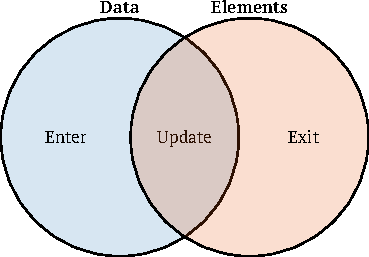
\includegraphics[width=0.5\textwidth]{fig/join}
	\caption{D3's \textit{data join}: Data points joined to existing elements produce the update (inner) selection. Leftover unbound data produce the enter selection (left), which represents missing elements. Likewise, any remaining unbound elements produce the exit selection (right), which represents elements to be removed. From \textit{Thinking with Joins} \cite{bostock2012join}.}
	\label{fig:join}
\end{figure}
%D3 goes down to the very basics in that it models what an update is at its core: the replacement of old data with new data. If we look at old data $O$ and new data $N$ as sets in a mathematical sense, their intersection $U = O \cap N$ are all the elements that need to be updated. $R = O \setminus U$ are all the old elements that are not part of the new elements and that need to be removed from the view. $A = N \setminus U$ are all the new elements that need to be added to the view. To understand d3, all one has to do is thus to start \textit{Thinking with Joins} \cite{bostock2012join}, which is an appealing blog article from D3's creator. The synchronization of the data join with the view is achieved through enter ($A$), update ($U$) and exit selections ($R$), in which one needs to append, update or remove DOM elements with the methods discussed above. this D3 specific software pattern 
The result of the join are enter, update and exit selections. New elements are added to the enter selection using \texttt{append()}, existing elements of the update selection modified using \texttt{style()} or \texttt{attr()}, and old elements of the exit selection removed with \texttt{remove()}.\footnote{To get familiar with D3's basics I suggest running and actively modifying small code snippets by yourself, which can be done directly in the web-based presentation of this interdisciplinary project:\\\url{http://www.adrian-haarbach.de/idp-graph-algorithms/presentation/slides.html\#/2/9}} This is the \textit{General Update Pattern, III} \cite{bostock2016general}, which is nicely illustrated using another of D3's strengths, transitions. These are used in our applicaiton to improve the understanding of the transitions between states of our algorithms. For the secondary visualization layer, we needed even more of D3's concepts, in particular axes and scales, because the numbers we want to visualize need to be converted to pixel coordinates that fit onto the screen. We recommend the books \cite{murray2013interactive,zhu2013data,meeks2015d3} as an introduction to these techniques.
%\subsection{JavaScript - the good parts}
%\subsection{SVG}

\section{Software design}\label{sec:design}% methods} %software algorithm design (high level)
We improved code quality and maintainability by adhering to object oriented programming best practices of \textit{high cohesion and low coupling} \refFigure{fig:coh}. The separation of the components now fits the \textit{Model-View-Controller (MVC)} design pattern \refFigure{fig:mvc}, which was already applied partially in previous work, even better. A good reference explaining how to apply these patterns using JavaScript is \cite{stefanov2010javascript}.
\begin{figure}
\centering
\begin{subfigure}[b]{0.3\textwidth}
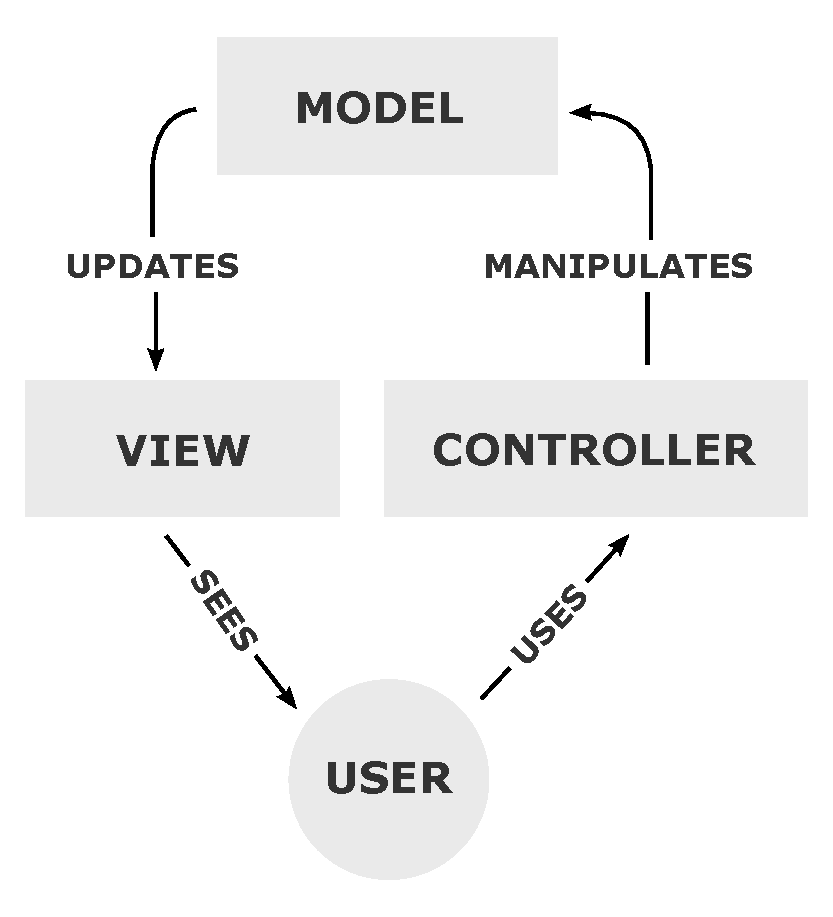
\includegraphics[width=\textwidth]{fig/MVC-Process}
	\caption{Model-View-Controller(MVC)\footnotemark}
	\label{fig:mvc}
\end{subfigure}
\begin{subfigure}[b]{0.68\textwidth}
\begin{small}
\begin{ssfont}
\begin{itemize}
\item Cohesion refers to the degree to which the elements of a class belong together, suggestion is all the related code should be close to each other, so we should strive for \textbf{high cohesion} and bind all related code together as far as possible. It has to do with the elements \textit{within} the class. %\textbf{High cohesion} means a class should do only one thing, but very well.
\item Coupling refers to the degree to which the different classes depend on each other, suggestion is all modules should be independent as far as possible, that's why \textbf{low coupling}. It has to do with the elements \textit{among} different classes. %\textbf{low coupling} suggest that class should have least possible dependencies.
\end{itemize}
\end{ssfont}
\end{small}
\caption{high cohesion, low coupling\footnotemark}
\label{fig:coh}
\end{subfigure}
\caption{Important design pattern and best practices in object oriented software engineering}
\label{fig:patterns}
\end{figure}
\footnotetext[10]{\url{https://en.wikipedia.org/wiki/Model-view-controller}}
\footnotetext{\url{http://stackoverflow.com/questions/14000762/low-in-coupling-and-high-in-cohesion}}

%%http://www.xyzws.com/scjp/SGS11/5/2
%Loose coupling makes it possible to:
%\begin{itemize}
%	\item Understand one class without reading others
%	\item Change one class without affecting others
%	\item Thus: improves maintainability
%\end{itemize}
%
%High cohesion makes it easier to:
%\begin{itemize}
%	\item Understand what a class or method does
%	\item Use descriptive names
%	\item Reuse classes or methods
%\end{itemize}

The improvements make it easier to reuse and extend the code in other projects. Thus, an early prototype of our implementation already served as a base for concurrent interdisciplinary projects \cite{fischer2016idp,feil2016idp}. These described some details of our implementation and its benefits over previous approaches in German. Here, we want to describe the overall concept and all improvements made in a unified manner and in English to serve as a good starting point for future projects. The chapter is organized into sections according to the MVC principle.

\subsection{Model}
%\item[Model] A major refactoring of the basic Graph class with the extension to arbitrary resources, easier algorithm state handling and new upload/download functionalities.
The graph Model of previous work was not very clean and thus substantially refactored and simplified while new features were added. It contained code concerning the naming, colouring and layout of nodes and edges and methods to draw them on Canvas and to detect clicks using coordinate comparisons. However, the Model should be oblivious to the actual graph drawing and interactions, since these belong to the View or the Controller. Moreover, the previous graph Model only allowed for a single scalar weight to be defined on edges. We extended it so that an arbitrary number of resources can be defined on both the edges and the nodes. This was especially needed for the SPPTW. Furthermore we added an associative array to nodes and edges to store the changing algorithm state, easing the replay functionality.

\renewcommand{\umldrawcolor}{black}
\colorlet{lightyellow}{yellow!20} %default color
\renewcommand{\umlfillcolor}{lightyellow}

\begin{figure}[htb!]
\centering
\begin{tikzpicture}
  \begin{class}[text width=7cm]{Graph}{0,0}
    \attribute{\underline{instance} : Graph}
    %\attribute{\underline{onLoadedCbFp} : [function]}
    \operation{getNodes() : [GraphNode]}
    \operation{getEdges() : [GraphEdge]}
    \operation{\underline{stringify(graph : Graph)} : String}
    \operation{\underline{parse(text : String)} : Graph}
    \operation{\underline{addChangeListener(callbackFp : function)}}
    %\operation{\underline{loadInstance(fileurl : String)}}
    %\operation{\underline{handleFileSelect(filename : String)}}
  \end{class}
  
  \begin{class}[text width=5.5cm]{GraphNode}{-5,-5}
    \attribute{resources : []}
    \attribute{state : \{\}}
    \attribute{x : number}
    \attribute{y : number}
    \operation{getInEdges() : [GraphEdge]}
    \operation{getOutEdges() : [GraphEdge]}
  \end{class}
  
  \begin{class}[text width=5.5cm]{GraphEdge}{4,-5}
    \attribute{resources : []}
    \attribute{state : \{\}}
    \operation{getStartNode() : GraphNode}
    \operation{getEndNode() : GraphNode}
  \end{class}
  
  \begin{class}[text width=3cm]{ResidualEdge}{1,-10}
  \end{class}
  
  \begin{class}[text width=2cm]{Label}{6,-10}
  \end{class}
  
  \composition{Graph}{nodes}{*}{GraphNode}
  \composition{Graph}{edges}{*}{GraphEdge}
  \association{GraphNode}{start,end}{1}{GraphEdge}{*}{in,out}
  \unidirectionalAssociation{GraphNode}{eligible}{*}{ResidualEdge}
  \association{GraphEdge}{}{1}{ResidualEdge}{1..2}{}
  \association{Label}{resident}{*}{GraphNode}{resident}{1}
  \unidirectionalAssociation{Label}{path}{*}{GraphEdge}
\end{tikzpicture}
\caption{UML class diagram for the Model. Static attributes and methods are \underline{underlined}. From a high-level perspective, we model a Graph as a composition of nodes and edges with associations between these two entities reflecting the network structure: Each GraphEdge has a start and an end node, while each GraphNode has an arbitrary number of incoming and outgoing edges. Arrays for resources denoted by [] and associate arrays for state variables denoted by \{\} are attributes of both nodes and edges. ResidualEdge and Label are two concepts that we needed for the implementation of our algorithms. These are primarily associated with GraphEdge, either 1:1 or 2:1 for the first or 1:n for the latter. For performance reason, we also established associations with GraphNode. A GraphNode can be queried for all its current outgoing eligible ResidualEdges, which is needed for applying a push operation. Label and GraphNode are associated bidirectionally: a Label needs to know its resident vertex so it can check path extensions easily for feasibility using the time-window of the vertex, while a GraphNode can be queried for all the Labels ending in it so we can apply dominance rules to them.}
%ResidualEdge and Label are concepts of our algorithms and are associated with GraphEdge and GraphNode.}
\label{fig:model}
\end{figure}

The new Graph class, composed by its subclasses GraphNode and GraphEdge, achieves high cohesion as can be seen in the UML diagram \refFigure{fig:model}. The static serialization and deserialization methods \underline{parse} and \underline{stringify} were extended to support arbitrary resource vectors. In previous work, the serialization capabilities were unaccessible to the end user. We provide a link to download a graph in its textual representation, which is backwards compatible to previous work. Additionally, a user can now locally upload a previously saved graph right from the browser using HTML5's FileReader \refSec{sec:script} capabilities. The previous raw AJAX \refSec{sec:basic} calls to load a saved sample graph from a server are now nicely wrapped in d3.text calls.

The loading of a graph, either from a local file or a remote server, is an asynchronous operation. According to \textit{MVC} \refFigure{fig:mvc}, the Model should update the View \refSec{sec:view} after any modifications to it, e.g. when another sample graph was selected or uploaded. We achieve \textit{low coupling} \refFigure{fig:coh} between the different components through the use of a static callback function registration method \underline{addChangeListener} \refFigure{fig:model}. All functions of the View that have been registered will be called after the graph has been loaded asynchronically without errors. The current graph is made available to the View and the Controller \refSec{sec:controller} via the static \underline{instance} object of Graph. This singleton pattern allows the Controller to easily access and manipulate the Model and the View to easily update its visual representation after any changes.  %To synchronize the current graph between GraphEditor and Algorithm, we employ a singleton pattern using the static Graph \underline{instance}.


\colorlet{lightgreen}{Akzent-Gruen!50}%tumblue3!40!lightyellow} %default color
%accentuating green} %SpringGreen}

\begin{figure}[htb!]
\centering
\hspace*{-0.5cm}%
\begin{tikzpicture}
  \renewcommand{\umlfillcolor}{tumblue4} %accentuating light blue}

  \begin{abstractclass}[text width=8cm]{GraphDrawer}{-3,0}
    \attribute{svg : <svg>}
    \operation{onNodesEntered(selection : [])}
    \operation{onNodesUpdated(selection : [])}
    \operation{onEdgesEntered(selection : [])}
    \operation{onEdgesUpdated(selection : [])}
    \operation{edgeText(d : GraphEdge) : String}
    \operation{nodeText(d : GraphNode) : String}
    \operation{nodeLabel(d : GraphNode) : String}
  \end{abstractclass}

  
  \begin{class}[text width=2.8cm]{LabelDrawer}{-4.9,-6}
  \end{class}
 
  \begin{class}[text width=5cm]{ResidualGraphDrawer}{3.5,-6}
  	\inherit{GraphDrawer}
  \end{class}
  

  \begin{class}[text width=2cm]{Logger}{-1,-6}
  \end{class}
  
  \renewcommand{\umlfillcolor}{lightgreen}
  
  \begin{class}[text width=3cm]{GraphEditor}{-8,-8}
    	\inherit{GraphDrawer}
  \end{class}
  
  \begin{class}[text width=5cm]{LabelSettingAlgorithm}{-3,-8}
  	\inherit{GraphDrawer}
  \end{class}

  \begin{class}[text width=5cm]{PushRelabelAlgorithm}{3,-8}
  	\inherit{GraphDrawer}
  \end{class}
  
  \begin{abstractclass}[text width=2.5cm]{Tab}{-3,-11}
  	\operation{init()}
  	\operation{activate()}
  	\operation{deactivate()}
  \end{abstractclass}
  
  \begin{class}[text width=3.5cm]{GraphEditorTab}{-7,-10}
    \inherit{Tab}
  	\operation{setGraphHandler()}
  \end{class}
  
  \begin{class}[text width=3.5cm]{AlgorithmTab}{2,-10}
    \inherit{Tab}
  	\operation{startFastForward()}
  	\operation{stopFastForward()}
  \end{class}
  
  \aggregation{LabelSettingAlgorithm}{}{}{LabelDrawer}
  \aggregation{PushRelabelAlgorithm}{}{}{ResidualGraphDrawer}
  
  
  \unidirectionalAssociation{AlgorithmTab}{}{}{Logger}
  \unidirectionalAssociation{LabelSettingAlgorithm}{}{}{AlgorithmTab}
  \unidirectionalAssociation{PushRelabelAlgorithm}{}{}{AlgorithmTab}
  \unidirectionalAssociation{GraphEditor}{}{}{GraphEditorTab}


\end{tikzpicture}
\caption{UML class diagram for View (blue) and Controller (green). The multiplicities are all 1:1 and thus not drawn. The abstract base class GraphDrawer of the View forms the basis for all graph-based visualizations. The Logger and the secondary visualization layers LabelDrawer and ResidualGraphDrawer are part of the View, but only the latter one displays a graph and thus extends the GraphDrawer. The abstract base class Tab of the Controller is extended to form a GraphEditorTab and an AlgorithmTab. Finally, the actual GraphEditor and the two implemented algorithms are associated with a Tab while inheriting from the GraphDrawer. Each algorithm has a secondary visualization layer, we model this relationship with an aggregation.}
\label{fig:viewcontroller}
\end{figure}



\subsection{View}\label{sec:view}
%	\item[View] A complete rewrite of the abstract GraphDrawer class for network visualization using D3.js and SVG instead of Canvas with the possibility to download it in vector format at any time. A Logger utility which allows to log algorithm execution messages with up to three indentation levels.
A complete rewrite of the graph visualization code was necessary because of the different drawing concepts of SVG vs. Canvas \refSec{sec:graphics}. D3.js is used extensively to achieve minimal code size with high expressiveness. The UML diagram \refFigure{fig:viewcontroller} shows all View classes in blue. The main result is the abstract GraphDrawer class, which should be used as a base class in all future projects. Full customization is easily possible by overwriting methods that will be called from inside of D3's \textit{data join} \refSec{sec:dthree}, in particular \texttt{onNodesEntered} and \texttt{onEdgesEntered} for the enter selections and \texttt{onNodesUpdated} and \texttt{onEdgesUpdated} for the update selections. For simple casess, it is sufficient to overwrite the methods \texttt{edgeText} and \texttt{nodeText} to customize the text that is drawn next to an edge or on top of a node. Per default these are the resource vector of the edge wrapped in \texttt{()} and possible constraints specified on the node wrapped in \texttt{[]}. The method \texttt{nodeLabel} returns the text displayed inside a node, typically a node's id. This method is typically overwritten to label start and end vertex with s and t. Any SVG based visualization can be saved to disk in vector format, for which styles and marker definitions are automatically inlined \refSec{sec:svgExport}. A Logger utility which allows to log algorithm execution messages with up to 3 indentation levels was furthermore developed. The log message data is joined with HTML list elements \texttt{<ol>} and \texttt{<ul>} using D3, which is not only limited to modifying SVG DOM, it can also handle HTML DOM. This class is very useful for development, but also for the final algorithm to display dynamic messages for each state of the algorithm and a complete trace of algorithm execution. The secondary visualization layers of each algorithm, namely the LabelDrawer and the ResidualGraphDrawer are also considered part of the View. The LabelDrawer \refFigure{fig:spprc} is used to visualize the Model Label by plotting its associated path with accumulated resource consumptions in a 2-dimensional height/cost chart together with the resident vertex' time window resource constraints as a rectangle. The ResidualGraphDrawer \refFigure{fig:maxflow} is used to display all outgoing residual edges of the currently active vertex which are considered for push or relabel operations. By limiting the display in such a way, we avoid the need for multiedges, because either only the forward or only the backward residual edge $e'$ of the original edge $e$ is shown at any time. The ResidualGraphDrawer allows to change the arrangement of nodes by changing the coordinate axes. While the original graph layout is obtained with y/x axes, we can rearrange the nodes with height/id or height/excess axes in order to visualize the concepts of height function and excess. This layered view with the height on the y axis allows to easily see which residual edges are eligible by checking if the difference of their node's heights is exactly one.

\subsection{Controller}\label{sec:controller}
%	\item[Controller] A new GraphEditor with support for modifying graphs with an arbitrary number of resources on nodes and edges. The new class Tab and a small refactoring improved future code reusability and simplified the reverse functionality and the synchronization between algorithm state and pseudocode lines.
	
	%A new way to save stateful data of the graph using JSON.stringify, which makes implementing the reverse functionality much easier. A new way to synchronize between the algorithm state (in the sense of a finite state machine), pseudocode lines, and their description using d3.
The UML diagram \refFigure{fig:viewcontroller} shows all Controller classes in green.
The basis of the Controller is the new abstract class Tab, which listens to changes of a Tab's visibility. The View of a Tab is defined in our HTML page with jQuery UI. The methods \texttt{init, activate} and \texttt{deactivate} should be overwritten to react to these visibility changes. A Tab is extended to form a GraphEditorTab and an AlgorithmTab with more specific functionality. The GraphEditorTab is used to wire together the events when another sample graph was selected or uploaded. These events trigger a call to the \texttt{setGraphHandler} method. This tab is used as an attribute of our new GraphEditor, which extends the GraphDrawer but is considered part of the Controller since it wires together different functionality. It comes with support for modifying graphs with an arbitrary number of resources on nodes and edges. This is achieved by rendering a number spinner HTML DOM element for each resource on top of the SVG network visualization, which allows to change the graph's underlying data Model conveniently. The AlgorithmTab connects the events of the fast forward jQuery UI buttons defined in the HTML page. Calls to the \texttt{startFastForward} and \texttt{stopFastForward} methods result from these events. It furthermore has a Logger instance of the View as an attribute, which allows to easily log and visualize algorithm execution. The AlgorithmTab is an attribute of the two main classes we developed for our algorithms, the LabelSettingAlgorithm and the PushRelabelAlgorithm. These extend the GraphDrawer and have an aggregation to their secondary visualization layers of LabelDrawer and ResidualGraphDrawer. The above design made it possible to separate most framework-related code from our main classes. If another algorithm is implemented in future work, one just has to copy and modify the LabelSettingAlgorithm or PushRelabelAlgorithm classes.



%\section{Installation}\label{sec:installation}

\chapter{Conclusion}\label{ch:6}
We developed two interactive web applications for advanced graph algorithms that can be accessed freely and furthermore made the source code available as open source to ease further extensions. We motivated the need for a secondary visualization layer concept and implemented it.

New technologies such as D3.js and SVG have been introduced as well as a lot of smaller new features implemented that make using the web application more interactive.

Over the years, a lot of web applications have been developed independently by different students. A lot of code was copied and partially modified, which resulted in a huge amount of duplication. The duplication of JavaScript files was minimized through the improved software design of this project, an early version of which \cite{feil2016idp} already applied to migrate previous, Canvas based implementations \cite{storz2013idp,velden2014idp,sefidgar2015idp,becker2015idp} to SVG.



\section{Future work}
\begin{itemize}
	\item 

	  the JavaScript architectureThe JavaScript ecosystem should be used to further improve 

\end{itemize}

% appendices (if appropriate)
%\appendix
%\chapter{Appendix}\label{ch:appendix}

In the appendix you can include \eg computer codes or further remarks which would disturb the flow of the main text. If you do not need an appendix, you can simply leave out this file (in which case you should also delete the \verb|\include| command in \texttt{thesis.tex}).
% all appendices behind backmatter will go without numbers
\backmatter

%List of Figures
%\listoffigures
%\vspace*{1.5cm}
%All figures in this document were created by the author using TikZ, the excellent \TeX-package by Till Tantau, see \cite{Tantau2007}.



%List of Tables
%\listoftables


%List of algorithms
% only in conjunction with algorithm2e
%\phantomsection% for hyperref
%\addcontentsline{toc}{chapter}{Algorithmenverzeichnis}%
%\markboth{Algorithmenverzeichnis}{Algorithmenverzeichnis}
%\listofalgorithms


%Algorithmenverzeichnis
% nur in Verbindung mit algorithm2e
%\phantomsection% fuer hyperref
%\addcontentsline{toc}{chapter}{Algorithmenverzeichnis}%
%\markboth{Algorithmenverzeichnis}{Algorithmenverzeichnis}
%\listofalgorithms

% Index
% Add index to table of contents
\addcontentsline{toc}{chapter}{Index}
\printindex

% Bibliography
\printbibliography[heading=bibintoc]

%In the final version, this should be empty and needn't be commented out. Someone who works sloppily should at least remember to comment out the fixme list, so that unfinished places are
%not so obvious for the examiners.
\listoffixmes
%
\end{document}
% ==============================================================================
% End of document
% ==============================================================================